\documentclass[11pt]{article}
\usepackage[margin=0.82in]{geometry}
\usepackage{amsmath,amssymb,booktabs,graphicx,float,microtype,tabularx,xcolor,enumitem,listings}
\usepackage[colorlinks=true,urlcolor=blue!55!black,linkcolor=blue!55!black]{hyperref}
\graphicspath{{../../output/reasoning/figures/}}
\definecolor{navy}{HTML}{1F4E78}
\definecolor{green}{HTML}{147D64}
\definecolor{coral}{HTML}{E07A5F}
\definecolor{codegray}{HTML}{F3F5F7}
\setlength{\parindent}{0pt}
\setlength{\parskip}{5pt}
\setlist{itemsep=2pt,topsep=3pt}
\lstset{basicstyle=\ttfamily\small,backgroundcolor=\color{codegray},frame=single,breaklines=true,columns=fullflexible}
\newcommand{\E}{\mathbb{E}}
\newcommand{\KL}{D_{\mathrm{KL}}}
\title{\textbf{Reasoning Models from an LLM}\\\large Detailed MATH 550 lecture notes and labs}
\author{Consumer-scale PyTorch track}
\date{August 2026}
\begin{document}
\maketitle
{\small\tableofcontents}
\newpage

\section{The main idea}
A reasoning model is still an autoregressive language model. It predicts one
token at a time. The difference is in its training data, objective, decoding
budget, and evaluation. We want the model to produce useful intermediate work,
obey a verifiable answer format, and spend additional computation only when that
computation improves a measured outcome.

This module begins with an existing language-capable model for the same reason a
reinforcement-learning course begins with a functioning neural network: our
teaching target is the new mechanism. The prior LLM module already constructs a
decoder-only transformer, byte-pair tokenizer, pretraining loop, SFT, reward
model, and PPO machinery from elementary PyTorch. Here we reuse that conceptual
foundation and implement math-reasoning post-training explicitly.

\subsection{Learning outcomes}
By the end, students can:
\begin{enumerate}
\item distinguish foundation pretraining, reasoning post-training, and
inference-time scaling;
\item define chain of thought as an observable generated sequence, distinguish
zero-shot and few-shot inputs, and place CoT correctly in prompting, SFT, and RL;
\item construct leakage-resistant train/validation/test splits for GSM8K;
\item implement an assistant-only SFT batch and explain every mask;
\item measure exact-answer accuracy, parse rate, pass@$k$, self-consistency, and
generation cost without conflating them;
\item derive REINFORCE, group-mean baselines, and the clipped GRPO loss;
\item separate baseline, advantage scaling, loss normalization, and importance correction;
\item compare GRPO, Dr. GRPO, RFT, MaxRL, PPO-style clipping, and GSPO;
\item implement verifiable rewards and identify reward hacking;
\item run revision-pinned Qwen or OLMo profiles with LoRA on CUDA, Apple MPS, or CPU; and
\item state what a tiny, single-seed experiment does and does not establish.
\end{enumerate}

\section{Chain of thought is a behavior, not a training algorithm}

Chain-of-thought (CoT) generation asks a language model to emit intermediate
reasoning text before its final answer.  Write the observable response as
\[
y=(z,a),\qquad
\pi_\theta(z,a\mid x)
=\prod_{t=1}^{|z|+|a|}\pi_\theta(y_t\mid x,y_{<t}),
\]
where $x$ is the problem and instruction, $z$ is the generated rationale or
scratchpad, and $a$ is the final answer.  CoT names the role of $z$.  It does
not specify whether parameters are updated, what loss is used, or where the
reasoning came from.

This definition answers two common questions.  First, an autoregressive LLM has
no separate ``CoT input port.''  The model always receives tokens and predicts
tokens.  Second, CoT belongs to no single training stage: it can be elicited at
inference, copied from demonstrations during SFT, generated and filtered for
another round of SFT, or sampled and rewarded during RL.

\subsection{What enters the context, and what the model must generate}

In direct prompting, the context contains a question and an answer-format
instruction.  In zero-shot CoT, it also asks for intermediate work:
\[
x=\text{system instruction}+\text{question}+\text{``reason step by step.''}
\]
The rationale $z$ is normally part of the model output.  In few-shot CoT, the
context additionally contains demonstration triples
\[
(x_1,z_1,a_1),\ldots,(x_K,z_K,a_K),x_{\rm new},
\]
so example rationales are input tokens while the new rationale and answer are
output tokens.  ``Is CoT input or output?'' therefore has a precise answer:
the new chain is output; demonstration chains may appear in the input context.

\begin{center}\small
\begin{tabularx}{\linewidth}{p{0.18\linewidth}p{0.25\linewidth}X p{0.14\linewidth}}
\toprule
Use of CoT & Input/context & Output or training target & Weight update? \\
\midrule
Prompting & question plus direct/CoT instruction; optionally example traces & model-generated $z,a$ & no \\
CoT SFT & question & supplied target rationale $z^*$ and answer $a^*$ & cross-entropy \\
Generate--filter--SFT & question; sometimes gold answer for rationalization & model traces filtered by correctness, then reused as targets & cross-entropy \\
CoT RL/RLVR & question plus sampling prompt & model-generated $z,a$ scored by reward/verifier & policy gradient \\
\bottomrule
\end{tabularx}
\end{center}

STaR is an important bridge rather than a synonym for RL.  It generates
rationales, retains or rationalizes successful ones, and fine-tunes by maximum
likelihood on those traces.  RFT/RAFT-style methods likewise convert sampled
successes into supervised targets.  A policy-gradient method instead keeps the
sampled response as an action trajectory and weights its score gradient by an
advantage.

\subsection{Why CoT can help---and what that evidence does not prove}

Generating $z$ can decompose one difficult conditional prediction into many
smaller ones, provide an external sequential workspace, and move the answer
distribution by conditioning on earlier intermediate tokens.  Few-shot traces
also specify a solution style and response contract.  These mechanisms explain
why CoT prompting can improve some multi-step tasks, especially for sufficiently
capable base models.  They do not imply that every extra token is useful, that
small models benefit, or that length itself is reasoning.

The emitted rationale is also not guaranteed to be a faithful causal record of
the network computation.  The answer may ignore parts of $z$, depend directly
on the prompt, rationalize an earlier guess, or remain correct despite a wrong
step.  Faithfulness is an intervention question: for example, does correcting,
removing, or perturbing a reasoning step predictably change the answer?  A
readable rationale is useful for auditing, but it is not privileged access to a
hidden human-like thought process.

\subsection{CoT under outcome-supervision RL}

Suppose the model samples $G$ responses
\[
(z_i,a_i)\sim\pi_{\rm old}(\cdot\mid x),\qquad i=1,\ldots,G,
\]
and an answer verifier returns $R_i=\mathbf 1[a_i=a^*]$.  A response-level
advantage $\hat A_i$ produces a token-factorized score gradient
\[
\hat A_i\nabla_\theta\log\pi_\theta(z_i,a_i\mid x)
=\hat A_i\sum_t\nabla_\theta\log\pi_\theta(y_{i,t}\mid x,y_{i,<t}).
\]
This is sequence-level credit broadcast across sampled tokens.  A positive
answer reinforces the sampled rationale and answer together; it does not prove
that every intermediate token caused success.  PPO/GRPO ratios can reweight or
saturate different tokens because their old-to-new probabilities differ, but a
single terminal advantage still gives them the same response-level sign.
Process rewards, a learned value function, step verification, counterfactual
edits, or tool execution can refine credit assignment.

RL also needs exploration support.  If the base/SFT model almost never samples a
correct parseable response, binary outcome groups tie at zero and group-relative
advantages vanish.  CoT prompting, SFT demonstrations, a stronger pretrained
model, curriculum, or denser checks can make successful trajectories reachable;
RL then redistributes probability among behaviors the policy can actually
sample.

\section{A four-week classroom sequence}
\begin{center}
\begin{tabularx}{\linewidth}{p{0.09\linewidth}p{0.23\linewidth}X}
\toprule
Week & Mechanism & Lab evidence \\
\midrule
1 & Elicit and evaluate CoT & Direct/zero-shot/few-shot inputs, parser, faithfulness, cost \\
2 & Teach worked solutions & Assistant-only SFT, LoRA, held-out loss, format ablation \\
3 & Spend test-time compute & Sampling, pass@$k$, majority vote, diversity and selection \\
4 & Optimize verifiable reward & Group advantages, clipping, reference KL, one online update \\
\bottomrule
\end{tabularx}
\end{center}
The order matters. If evaluation is unreliable, reinforcement learning optimizes
the wrong target faster. If SFT has not taught a parseable answer contract, most
reward groups are uninformative. If sampling lacks diversity, a group-relative
objective receives zero advantages.

\section{From next-token prediction to worked solutions}
Let the prompt $x$ contain the system instruction and math problem, and let
$y=(y_1,\ldots,y_T)$ contain a written solution followed by a final answer. The
model factorizes
\[
\pi_\theta(y\mid x)=\prod_{t=1}^{T}\pi_\theta(y_t\mid x,y_{<t}).
\]
The ordinary negative log likelihood is
\[
-\log\pi_\theta(y\mid x)=-\sum_t\log\pi_\theta(y_t\mid x,y_{<t}).
\]
For instruction tuning, we do not want to train the model to reproduce the
system prompt or question. Define a mask $m_t$ that is one only at assistant
response tokens. The course loss is
\[
\mathcal L_{\mathrm{SFT}}(\theta)
=-\frac{\sum_t m_t\log\pi_\theta(y_t\mid x,y_{<t})}{\sum_t m_t}.
\]
In code, prompt and padding labels are \texttt{-100}; PyTorch cross entropy
ignores them. The input still contains the prompt, because response predictions
condition on it. Masking a token from the loss is not the same as masking it from
attention.

\subsection{Why written work can help}
Intermediate tokens can decompose a difficult mapping into shorter conditional
steps. They also supply many supervised targets per problem. But useful output
does not prove faithful internal computation. A model may rationalize a guess,
copy a familiar template, or make a wrong step that happens to cancel later.
Treat a rationale as an auditable artifact, not privileged access to thought.

\section{Parameter-efficient adaptation with LoRA}
Full fine-tuning stores gradients and optimizer states for every parameter. LoRA
freezes a pretrained matrix $W_0\in\mathbb R^{d_{\rm out}\times d_{\rm in}}$ and
learns
\[
\Delta W=\frac{\alpha}{r}BA,
\quad A\in\mathbb R^{r\times d_{\rm in}},\quad
B\in\mathbb R^{d_{\rm out}\times r},\quad r\ll d.
\]
The forward map is $h=W_0x+\Delta Wx$. The local rank-4 adapter updates only
0.443\% of the 496.2M parameters. The recommended rank-16 preset adds capacity
while remaining practical on a consumer accelerator.

LoRA is not automatically better than full fine-tuning. It is a resource choice.
Rank, target modules, context length, batch accumulation, and learning rate form
an experimental design. The course targets attention projections and feed-forward
projections; an ablation can restrict LoRA to query and value maps.

\section{Data: GSM8K without test leakage}
GSM8K contains 7,473 training and 1,319 test problems. Each training answer has
human-written steps and a final line beginning with \texttt{\#\#\#\#}. The
problems require roughly two to eight elementary arithmetic steps. The module
downloads raw JSONL from commit
\texttt{3101c7d5072418e28b9008a6636bde82a006892c} of the official repository
and checks SHA-256. It does not depend on a Kaggle mirror.

The official test set remains untouched until final evaluation. A deterministic
512-row validation set comes from training. Model selection, early stopping, and
prompt changes must use that internal validation set. Looking at test errors and
then changing the prompt is test tuning even if no gradient was computed.

\begin{figure}[H]\centering
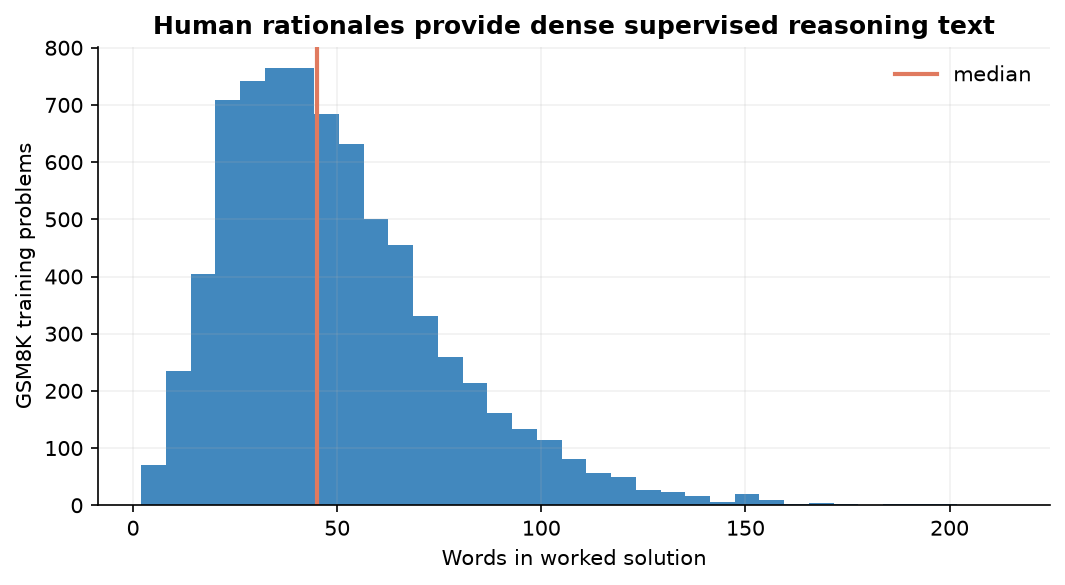
\includegraphics[width=0.86\linewidth]{rationale_length_distribution.png}
\caption{GSM8K training rationales have median 45 words, mean 49.7, and 90th percentile 85.}
\end{figure}

The loader removes calculator annotations of the form
\texttt{<<expression=result>>}. The visible result following the annotation is
retained. This produces natural worked text while keeping the authoritative
numeric answer. A different experiment could retain annotations and implement a
calculator tool; that would be a tool-use lesson, not the default here.

\section{Evaluation is part of the model}
\subsection{A robust but narrow answer contract}
The preferred response ends with \texttt{\#\#\#\# number}. The extractor tries:
\begin{enumerate}
\item the last marked answer;
\item a boxed or explicitly labeled final answer; then
\item the last numeric expression as a diagnostic fallback.
\end{enumerate}
It strips currency and thousands separators and normalizes decimals, fractions,
and percentages. Exact-answer reward is reliable only inside this contract. It
does not judge whether the units, assumptions, or reasoning are sound.

For $n$ problems with gold $a_i^*$ and parsed prediction $\hat a_i$,
\[
\widehat{\mathrm{Acc}}=\frac1n\sum_{i=1}^n\mathbf 1[\hat a_i=a_i^*].
\]
Report parse rate separately. Counting an unparseable response as wrong is
appropriate for accuracy; hiding the parse rate conceals an engineering failure.

\subsection{Uncertainty}
For a tiny binomial probe, a Wilson interval is more stable than
$\hat p\pm1.96\sqrt{\hat p(1-\hat p)/n}$ near zero or one. With $z=1.96$,
\[
\mathrm{center}=\frac{\hat p+z^2/(2n)}{1+z^2/n},\qquad
\mathrm{half}=\frac{z}{1+z^2/n}
\sqrt{\frac{\hat p(1-\hat p)}n+\frac{z^2}{4n^2}}.
\]
The local base and SFT intervals overlap widely. That is why the report calls the
result a pipeline probe.

\section{Inference-time scaling}
Greedy decoding chooses the largest next-token probability at each step. Sampling
with temperature $\tau$ uses
\[
p_\tau(v)=\frac{\exp(z_v/\tau)}{\sum_u\exp(z_u/\tau)}.
\]
Sampling $K$ paths can uncover a correct solution the greedy path misses.
Pass@$K$ is the fraction of problems with at least one correct sample. It is an
oracle diagnostic because it uses the gold answer after generation.

Self-consistency chooses the most frequent extracted answer:
\[
\hat a_{\rm SC}=\arg\max_a\sum_{k=1}^K\mathbf 1[a_k=a].
\]
It works when correct paths occupy a substantial portion of the distribution.
Correlated errors can win unanimously. A tie rule must be deterministic; the
course implementation uses the first occurring tied answer.

\begin{figure}[H]\centering
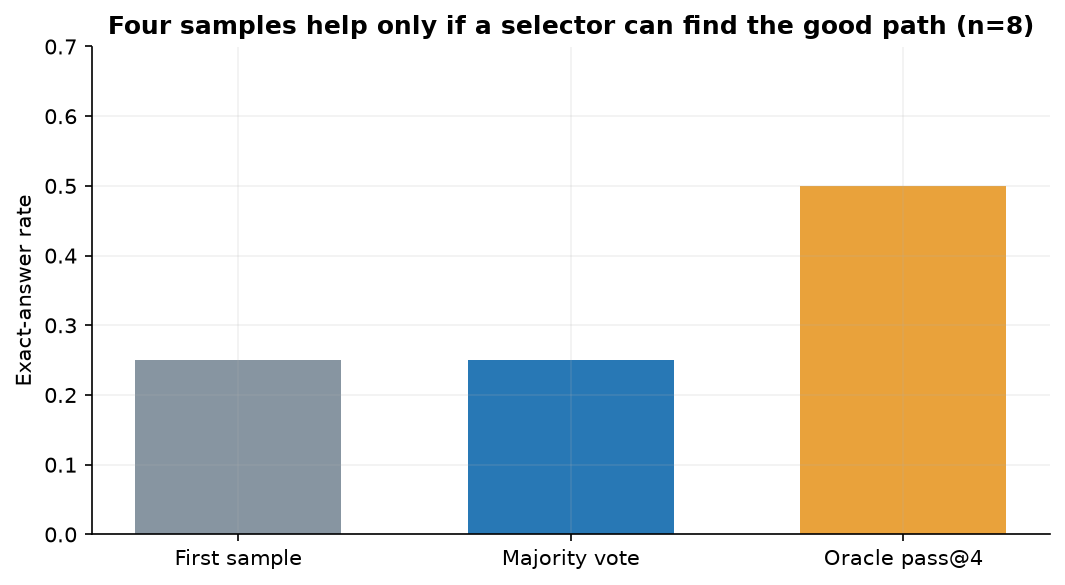
\includegraphics[width=0.78\linewidth]{inference_time_scaling.png}
\caption{On eight problems, four samples doubled oracle coverage but did not improve majority selection.}
\end{figure}

The important comparison is compute matched. Four samples cost roughly four
times as many generated tokens as one, although batched GPU throughput may reduce
wall time. Compare quality against total generated tokens, latency, and energy,
not only number of questions.

\section{Alignment is a family of data--objective pairs}

``Alignment'' is not synonymous with reinforcement learning.  In this course it
means modifying a pretrained model toward an explicit behavior specification
and auditing both the intended and unintended changes.  Four common pairs are:
\begin{center}
\begin{tabularx}{\linewidth}{p{0.17\linewidth}p{0.25\linewidth}X}
\toprule
Method & Feedback & What is optimized \\
\midrule
SFT & Demonstration $(x,y^*)$ & Response-token log likelihood \\
Reward model & Ranked pair $(y_w,y_l)$ & Bradley--Terry preference likelihood \\
DPO & Ranked pair plus reference & Offline preference likelihood expressed as policy ratios \\
RLHF/RLVR & Online rollout plus learned/hard reward & Expected reward, usually with a reference or update constraint \\
\bottomrule
\end{tabularx}
\end{center}
RLHF typically learns a reward model from human preferences.  RLVR uses a
verifier---for example exact arithmetic---so the scalar reward is cheap and
repeatable but only as good as its parser and specification.  A model can
maximize either reward while becoming worse on omitted qualities.

A common KL-regularized target is
\[
\max_\pi\;\E_{y\sim\pi(\cdot\mid x)}[R(x,y)]
-\beta\KL\!\left(\pi(\cdot\mid x)\|\pi_{\rm ref}(\cdot\mid x)\right).
\]
For an unconstrained distribution at one prompt, Lagrange multipliers give
$\pi^*(y\mid x)\propto\pi_{\rm ref}(y\mid x)e^{R(x,y)/\beta}$.  DPO substitutes
this relation into a Bradley--Terry model.  For preferred $y_w$ and rejected
$y_l$, its per-pair loss is
\[
-\log\sigma\!\left(\beta\left[
\log\frac{\pi_\theta(y_w\mid x)}{\pi_{\rm ref}(y_w\mid x)}-
\log\frac{\pi_\theta(y_l\mid x)}{\pi_{\rm ref}(y_l\mid x)}
\right]\right).
\]
DPO is offline and avoids a rollout loop; RLVR directly explores the current
policy and can discover new correct solutions.  They answer different data
availability questions rather than forming a universal ranking.

\section{Deriving language-model policy gradients}

For prompt distribution $x\sim\rho$, response $y\sim\pi_\theta(\cdot\mid x)$,
and verifier reward $R(x,y)$,
\[
J(\theta)=\E_{x\sim\rho}\E_{y\sim\pi_\theta}[R(x,y)].
\]
Applying $\nabla p=p\nabla\log p$ gives
\begin{align}
\nabla J(\theta)
&=\E_{x,y}[R(x,y)\nabla\log\pi_\theta(y\mid x)]\\
&=\E_{x,y}\left[R(x,y)\sum_{t=1}^{|y|}
\nabla\log\pi_\theta(y_t\mid x,y_{<t})\right].
\end{align}
The prompt-plus-prefix is the RL state; the next token is the action; the
verifier supplies a terminal return.  We do not differentiate through sampled
tokens or the verifier.  The gradient comes from the log probability assigned
to actions that were actually sampled.

Subtracting any $b(x)$ independent of $y$ is unbiased because
$\E_y[\nabla\log\pi_\theta(y\mid x)]=0$.  The empirical group mean used by GRPO
is subtler because it contains the current response.  For $G$ iid responses,
\[
\E\left[\frac1G\sum_{j=1}^G(R_j-\bar R)
\nabla\log\pi_\theta(Y_j\mid x)\right]
=\frac{G-1}{G}\nabla J_x(\theta).
\]
Thus it preserves the direction up to a finite-group scale before any further
normalization.

\section{GRPO is an estimator design space}

For one prompt group,
\[
\bar R=\frac1G\sum_jR_j,\qquad
s=\sqrt{\frac1G\sum_j(R_j-\bar R)^2}.
\]
The implementation makes three independent choices visible:
\begin{center}
\begin{tabularx}{\linewidth}{p{0.18\linewidth}p{0.20\linewidth}p{0.20\linewidth}X}
\toprule
Name & Baseline & Advantage scale & Token-loss denominator \\
\midrule
GRPO & group mean & group std & each sequence length \\
GRPO-constant & group mean & group std & fixed $Z$ \\
Dr. GRPO & group mean & none & fixed $Z$ \\
RFT / expert iteration & none & none & fixed $Z$; zero-reward samples vanish \\
MaxRL & group mean & group mean & fixed $Z$ in this controlled lab \\
\bottomrule
\end{tabularx}
\end{center}
The standard sequence-normalized objective has the form
\[
\widehat g_{\rm seq}=\frac1{BG}\sum_{i,j}\frac{A_{ij}}{L_{ij}}
\sum_{t=1}^{L_{ij}}\nabla\log\pi_\theta(y_{ijt}\mid x_i,y_{ij,<t}),
\]
so every completion gets equal total weight.  Constant normalization instead
uses
\[
\widehat g_{\rm const}=\frac1Z\sum_{i,j,t}A_{ij}
\nabla\log\pi_\theta(y_{ijt}\mid x_i,y_{ij,<t}),
\]
so a longer response contributes more selected-token terms.  Neither choice is
length neutral: one can favor short solutions per token; the other can favor
long solutions in total.  The denominator is part of the algorithm.

For binary rewards and an infinite group, let prompt success probability be
$\eta(x)$.  Ignoring the common finite-$G$ factor, Dr. GRPO weights prompts by
$1$, standard-deviation GRPO by $1/\sqrt{\eta(1-\eta)}$, and MaxRL by
$1/\eta$.  Standard GRPO emphasizes both very easy and very hard prompts;
MaxRL strongly emphasizes hard prompts.  These are surrogate prompt
distributions, not mere numerical stabilization.

\begin{figure}[H]\centering
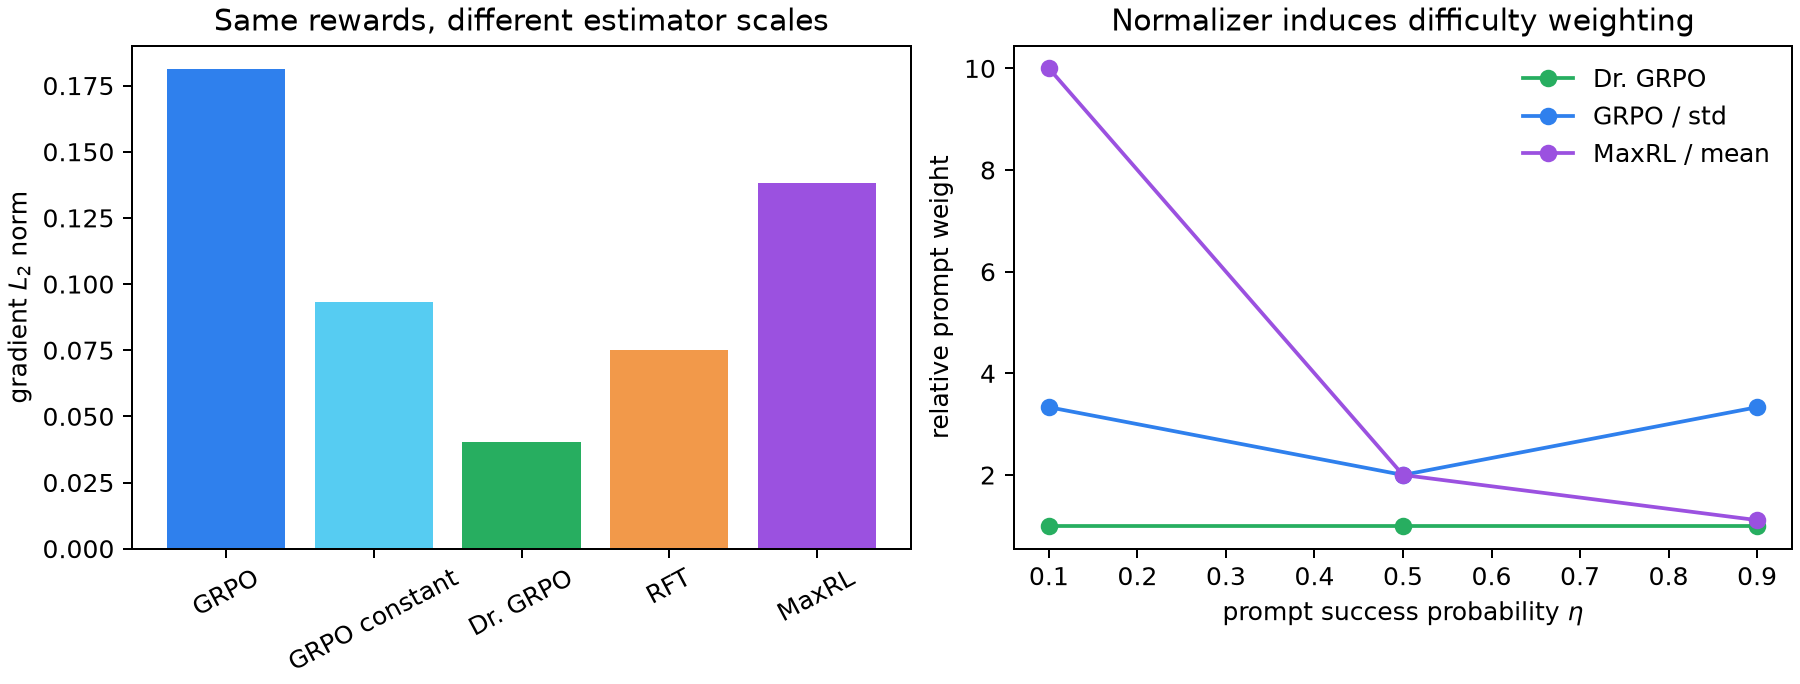
\includegraphics[width=\linewidth]{rlvr_estimator_tradeoffs.png}
\caption{Fixed-tensor audit from \texttt{make audit-rlvr}.  It verifies
mechanics and induced weighting, not downstream model quality.}
\end{figure}

If every reward in a mean-baseline group ties, every advantage is exactly zero.
Such sequences can be pruned without changing the gradient.  In RFT, every
zero-reward sample can be pruned.  This saves compute but also exposes a hard
limit: optimization cannot recover a signal that sampling and grading never
produced.

\section{On-policy, stale rollouts, clipping, and GSPO}

On-policy means the responses were drawn from the policy whose gradient is
being estimated.  If $y\sim\pi_0$ is stale, exact sequence importance sampling
uses
\[
w(y)=\frac{\pi_\theta(y\mid x)}{\pi_0(y\mid x)}
=\prod_t\rho_t,\qquad
\rho_t=\exp(\log\pi_\theta(y_t\mid\cdot)-\log\pi_0(y_t\mid\cdot)).
\]
The full product corrects the sampling distribution but can have enormous
variance.  Token-level PPO/GRPO replaces the product by a separate $\rho_t$ in
each token term.  This reduces variance but is biased: the prefix and suffix
still come from $\pi_0$.  It can be understood as optimizing a surrogate policy
that swaps in the current policy at only one token position.

The clipped token surrogate is
\[
L=\min\{\rho_tA,\operatorname{clip}(\rho_t,1-\epsilon,1+\epsilon)A\}.
\]
In the live region,
\[
\nabla_\theta(\rho_tA)=\rho_tA\nabla_\theta
\log\pi_\theta(y_t\mid x,y_{<t}).
\]
Thus every response token is reweighted separately even if outcome supervision
broadcasts the same response advantage $A$.  When $A>0$, gradient vanishes
above $1+\epsilon$; when $A<0$, it vanishes below $1-\epsilon$.  A ratio outside
the window on the opposite side remains active.  Clipping is a biased guardrail,
not a proof of a KL trust region.
CISPO instead upper-clips the importance weight directly.  The course includes
it as an optional code path so students can separate ``which ratio'' from
``which clipping rule.''

GSPO shares one geometric-mean ratio across a completion,
\[
s(y)=\exp\left(\frac1{|y|}\sum_t\log\rho_t\right),
\]
then applies the same signed clipping pattern to $sA$.  It includes sequence
context in the ratio while avoiding the exponential-scale product.  The
geometric mean and clipping both introduce bias.  There is no universally best
point on the bias--variance spectrum; staleness, response length, and policy
drift determine the tradeoff.

This also locates PPO on the on/off-policy spectrum.  Rollouts are on-policy at
the moment $\pi_0$ generates them.  Multiple optimizer epochs make them stale
relative to the live $\pi_\theta$, so token ratios perform limited action-level
correction.  The prefixes and their visitation distribution still came from
$\pi_0$, and clipping deliberately changes the correction.  PPO is therefore
best described as near-on-policy optimization with bounded data reuse, not as a
fully off-policy replay algorithm.

\subsection{Reference regularization}
Reward alone can push the adapter away from useful language behavior. The frozen
base model is a reference. Let $f=\log\pi_{\rm ref}-\log\pi_\theta$. The course
uses the nonnegative estimator
\[
k_3(f)=e^f-f-1\geq0,
\]
and total loss
\[
\mathcal L_{\rm GRPO}=\mathcal L_{\rm policy}+\beta\E[k_3].
\]
Only response tokens enter either term. The old policy and reference log
probabilities are detached. The current log probabilities retain gradients.

\section{Verifiable reward and its failure modes}
The course reward is exact answer plus a small format bonus. It is intentionally
transparent:
\[
R=1.0\,\mathbf1[\hat a=a^*]+0.1\,\mathbf1[\text{marked format}],
\]
and an unparseable output receives $-0.1$. The 0.1 bonus is smaller than answer
correctness so formatting cannot outweigh a correct answer.

Failure modes include:
\begin{itemize}
\item \textbf{Parser exploitation:} emit multiple numbers or malformed markup that
the extractor reads favorably.
\item \textbf{Outcome-process mismatch:} obtain the right number with invalid work.
\item \textbf{Sparse groups:} all answers are wrong, so every advantage is zero.
\item \textbf{Length drift:} the model produces long text because another signal
correlates with reward.
\item \textbf{Distribution narrowing:} repeated policy updates remove useful
diversity and exploration.
\item \textbf{Memorization:} benchmark-like templates look like general reasoning.
\end{itemize}
Mitigations include strict parsing tests, process checks on sampled rationales,
reference KL, held-out transfer, reward-component logging, length diagnostics,
and adversarial cases.

\section{Implementation map}
\begin{center}
\begin{tabularx}{\linewidth}{p{0.36\linewidth}X}
\toprule
File & Responsibility \\
\midrule
\texttt{reasoning/data.py} & Strict GSM8K/SVAMP loaders, answer normalization, chat prompts, response masks \\
\texttt{reasoning/evaluation.py} & Exact records, Wilson intervals, majority vote, pass@$k$, rewards \\
\texttt{core/alignment.py} & Shared baselines, advantage scales, denominators, token/sequence ratios, clipping, KL \\
\texttt{reasoning/objectives.py} & Shifted response log probabilities and reasoning-facing objective API \\
\texttt{reasoning/modeling.py} & Device policy, three revision-pinned open-model profiles, LoRA, frozen reference \\
\texttt{reasoning/training.py} & Explicit AdamW SFT loop, generation, configurable online RLVR update \\
\texttt{experiments/reasoning/} & Thin download, train, evaluate, summarize, and plot drivers \\
\bottomrule
\end{tabularx}
\end{center}

Neural primitives remain PyTorch/Hugging Face modules. The teaching code owns
the masks, losses, rewards, rollout grouping, evaluation, and optimizer loops.
This follows the project rule: expose the mechanism under study without
reimplementing tensor autograd or production transformer kernels.

\section{Running the module}
\begin{lstlisting}
uv sync --locked --extra reasoning
make download-reasoning-data
make test-reasoning
make smoke-reasoning
make audit-rlvr

# Short real-model lab
uv run --extra reasoning python -m experiments.reasoning.sft \
  --preset quick --device auto

# Untouched GSM8K evaluation
uv run --extra reasoning python -m experiments.reasoning.evaluate \
  --dataset gsm8k --adapter checkpoints/reasoning/sft-quick/adapter \
  --device auto --limit 128 --samples 1 --output-name sft_quick_128

# Online verifiable-reward extension
uv run --extra reasoning python -m experiments.reasoning.grpo \
  --preset quick --adapter checkpoints/reasoning/sft-quick/adapter \
  --device auto --updates 10 --prompts-per-update 2 --variant dr-grpo

# Stronger, opt-in math checkpoint (about 3.1 GB of weights)
uv run --extra reasoning python -m experiments.reasoning.sft \
  --preset quick --device auto --model-profile qwen-math-1.5b
\end{lstlisting}
\texttt{auto} chooses CUDA, then MPS, then CPU. Explicit unavailable CUDA or MPS
requests fail. MPS uses float32 for stability. CUDA uses bfloat16 when supported,
otherwise float16. Model weights are revision pinned and Apache-2.0 licensed.

\section{Measured evidence and interpretation}
The local 20-step rank-4 run used 128 training and 64 validation examples.
Validation token loss fell from 1.174 to 0.740 in 14.24 seconds on Apple M2 MPS.
On 16 fixed test rows, exact answers changed from 2 to 5, marked-format compliance
from 0 to 16, and mean response length from 189.2 to 82.4 tokens.

\begin{figure}[H]\centering
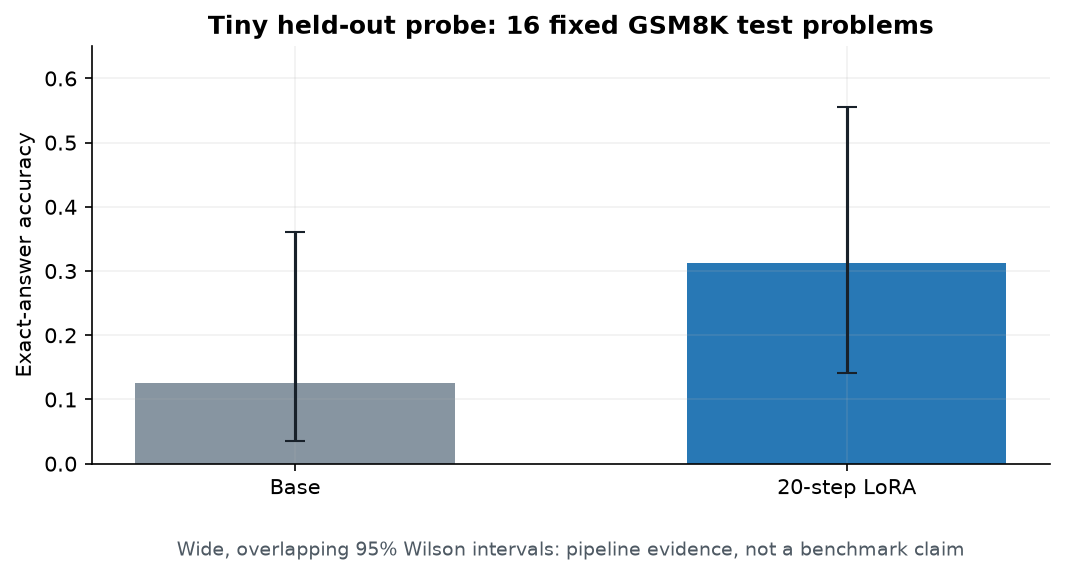
\includegraphics[width=0.72\linewidth]{tiny_accuracy_probe.png}
\caption{The intervals make the evidence boundary visible.}
\end{figure}

\begin{figure}[H]\centering
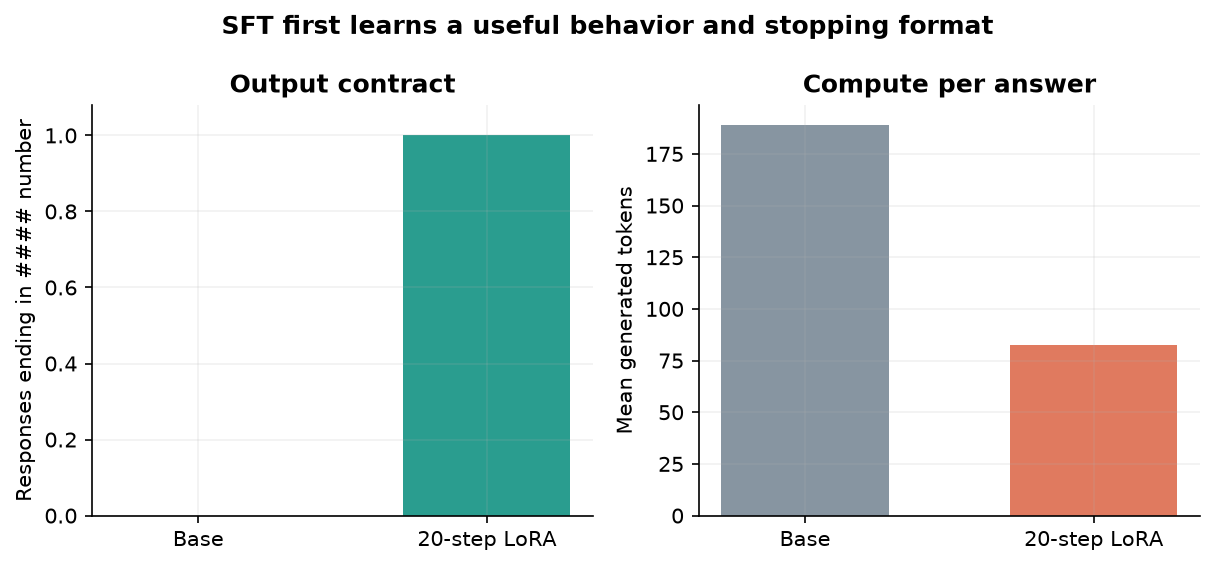
\includegraphics[width=0.94\linewidth]{format_and_length.png}
\caption{The strongest local conclusion is behavioral: the model learned the requested output contract.}
\end{figure}

One online GRPO update sampled two responses with equal reward. The group
advantages were exactly zero, so the policy signal vanished; the finite update
contained only the reference penalty. This is an important correctness check and
a warning: increasing optimizer updates cannot compensate for uninformative
sampling.

\section{Choosing a base model on one consumer device}
The model registry separates a fast mechanism check from stronger-capability
tracks.  Every entry has an immutable 40-character Hugging Face revision in
\texttt{data/reasoning/sources.json}.
\begin{center}
\begin{tabularx}{\linewidth}{p{0.20\linewidth}p{0.29\linewidth}p{0.16\linewidth}X}
\toprule
Profile & Checkpoint & Approx. weights & Recommended role \\
\midrule
\texttt{qwen-0.5b} & Qwen2.5-0.5B-Instruct & 0.99 GB & default smoke and code tracing \\
\texttt{qwen-math-1.5b} & Qwen2.5-Math-1.5B-Instruct & 3.09 GB & stronger math SFT/evaluation on high-memory MPS, 4090, or Colab \\
\texttt{olmo2-1b-instruct} & OLMo-2-0425-1B-Instruct & 2.98 GB & open-science comparison with released training artifacts \\
\bottomrule
\end{tabularx}
\end{center}
The OLMo Instruct checkpoint already received SFT, DPO, and RLVR.  It is useful
for inference and systems comparison, but it is not a clean pre-RL baseline for
claiming that this course's RLVR created its existing reasoning ability.  Qwen
Math is also domain-specialized.  Comparisons must therefore state checkpoint
history, not only parameter count.

\section{How to scale the experiment responsibly}
Use the following order:
\begin{enumerate}
\item time 20 SFT updates on the target device;
\item choose a step budget from observed seconds per update;
\item log internal validation loss and a fixed validation generation panel;
\item run the untouched GSM8K test once after choices are frozen;
\item repeat at least three seeds before claiming a mean effect;
\item evaluate SVAMP transfer and classify errors;
\item compare greedy, sampling, and majority vote at matched token budgets; and
\item add GRPO only after reward groups show nonzero variance.
\end{enumerate}
The included MPS preset uses context 384, rank 16, batch 1, accumulation 8, and
800 optimizer steps. The Colab preset uses context 512, batch 4, accumulation 8,
and 1,200 steps. Both are teaching targets, not runtime promises.

\section{Limitations and responsible claims}
GSM8K measures a narrow form of English grade-school arithmetic. Exact numeric
answers ignore units and proof validity. Rationales can be unfaithful. A 0.5B
model has limited capacity, and one small adapter may forget useful behaviors.
The short measured probe uses one seed and a fixed test prefix. The first 16 rows
are not a random confidence sample from all possible math tasks.

Avoid these claims: ``the model learned to reason,'' ``chain of thought is an
explanation of internal cognition,'' or ``GRPO guarantees self-improvement.''
Prefer: ``under this prompt and parser, the checkpoint increased exact answers
on this held-out set,'' ``sampled rationales provide inspectable intermediate
text,'' and ``the objective produced finite gradients with nonzero group
advantages.''

\section{References}
\footnotesize
\begin{itemize}\setlength{\itemsep}{0pt}\setlength{\parskip}{0pt}
\item Cobbe et al. (2021), \emph{Training Verifiers to Solve Math Word Problems}, \url{https://arxiv.org/abs/2110.14168}.
\item Wei et al. (2022), \emph{Chain-of-Thought Prompting Elicits Reasoning in Large Language Models}, \url{https://arxiv.org/abs/2201.11903}.
\item Kojima et al. (2022), \emph{Large Language Models are Zero-Shot Reasoners}, \url{https://arxiv.org/abs/2205.11916}.
\item Wang et al. (2022), \emph{Self-Consistency Improves Chain of Thought Reasoning in Language Models}, \url{https://arxiv.org/abs/2203.11171}.
\item Zelikman et al. (2022), \emph{STaR: Bootstrapping Reasoning With Reasoning}, \url{https://arxiv.org/abs/2203.14465}.
\item Lanham et al. (2023), \emph{Measuring Faithfulness in Chain-of-Thought Reasoning}, \url{https://arxiv.org/abs/2307.13702}.
\item Patel et al. (2021), \emph{Are NLP Models really able to Solve Simple Math Word Problems?}, \url{https://aclanthology.org/2021.naacl-main.168/}.
\item Shao et al. (2024), \emph{DeepSeekMath}, \url{https://arxiv.org/abs/2402.03300}.
\item DeepSeek-AI (2025), \emph{DeepSeek-R1}, \url{https://arxiv.org/abs/2501.12948}.
\item Stanford CS336 (2026), \emph{Assignment 5: Alignment}, \url{https://github.com/stanford-cs336/assignment5-alignment}; repository revision \texttt{c2734a2} and handout SHA-256 are pinned in the manifest.
\item Schulman et al. (2017), \emph{Proximal Policy Optimization Algorithms}, \url{https://arxiv.org/abs/1707.06347}.
\item Rafailov et al. (2023), \emph{Direct Preference Optimization}, \url{https://arxiv.org/abs/2305.18290}.
\item Liu et al. (2025), \emph{Understanding R1-Zero-Like Training: A Critical Perspective}, \url{https://arxiv.org/abs/2503.20783}.
\item Tajwar et al. (2026), \emph{Maximum Likelihood Reinforcement Learning}, \url{https://arxiv.org/abs/2602.02710}.
\item Zheng et al. (2025), \emph{Group Sequence Policy Optimization}, \url{https://arxiv.org/abs/2507.18071}.
\item Raschka (2025), \emph{Build A Reasoning Model (From Scratch)} code, \url{https://github.com/rasbt/reasoning-from-scratch}.
\item Qwen team, Qwen2.5-0.5B-Instruct model card, \url{https://huggingface.co/Qwen/Qwen2.5-0.5B-Instruct}; revision \texttt{7ae5576} is pinned in the manifest.
\item Qwen team, Qwen2.5-Math-1.5B-Instruct model card, \url{https://huggingface.co/Qwen/Qwen2.5-Math-1.5B-Instruct}; revision \texttt{aafeb0f} is pinned.
\item Ai2, OLMo-2-0425-1B-Instruct model card, \url{https://huggingface.co/allenai/OLMo-2-0425-1B-Instruct}; revision \texttt{48d788e} is pinned.
\end{itemize}
\end{document}
